\documentclass[a4paper]{report}

\usepackage[nottoc,numbib]{tocbibind}
\usepackage{graphicx}

\begin{document}

\title{Title}
\author{Fredrik Appelros \and Carl Ekerot}
\date{\today}
\maketitle

\begin{abstract}
An abstract is a brief summary of a research article, thesis, review,
conference proceeding or any in-depth analysis of a particular subject or
discipline, and is often used to help the reader quickly ascertain the paper's
purpose.
\end{abstract}

\tableofcontents

\chapter{Introduction}

\section{Background}

\section{Related work}
Here is a discussion about related work. As an example here is a citation
\cite{cui07}.

\chapter{Method}

\section{Approach}

\section{Clustering}

\subsection{Cluster theory}

\subsubsection{K-means - Example from SciKit-Learn}

\subsection{Features}

\subsubsection{High dimensional data}

\subsubsection{PCA - Example DNS traffic}

\subsection{Hierarchical clustering}

\subsubsection{UPGMA - Example DNS traffic (tree)}

\subsection{Density-based clustering}

\subsubsection{DBSCAN - Example DNS traffic}

\subsubsection{OPTICS}

\paragraph{Cluster extraction}

\section{Field analysis}

\subsection{Byte distribution}

\subsection{Field classes}

\subsection{RANSAC}

\begin{figure}
    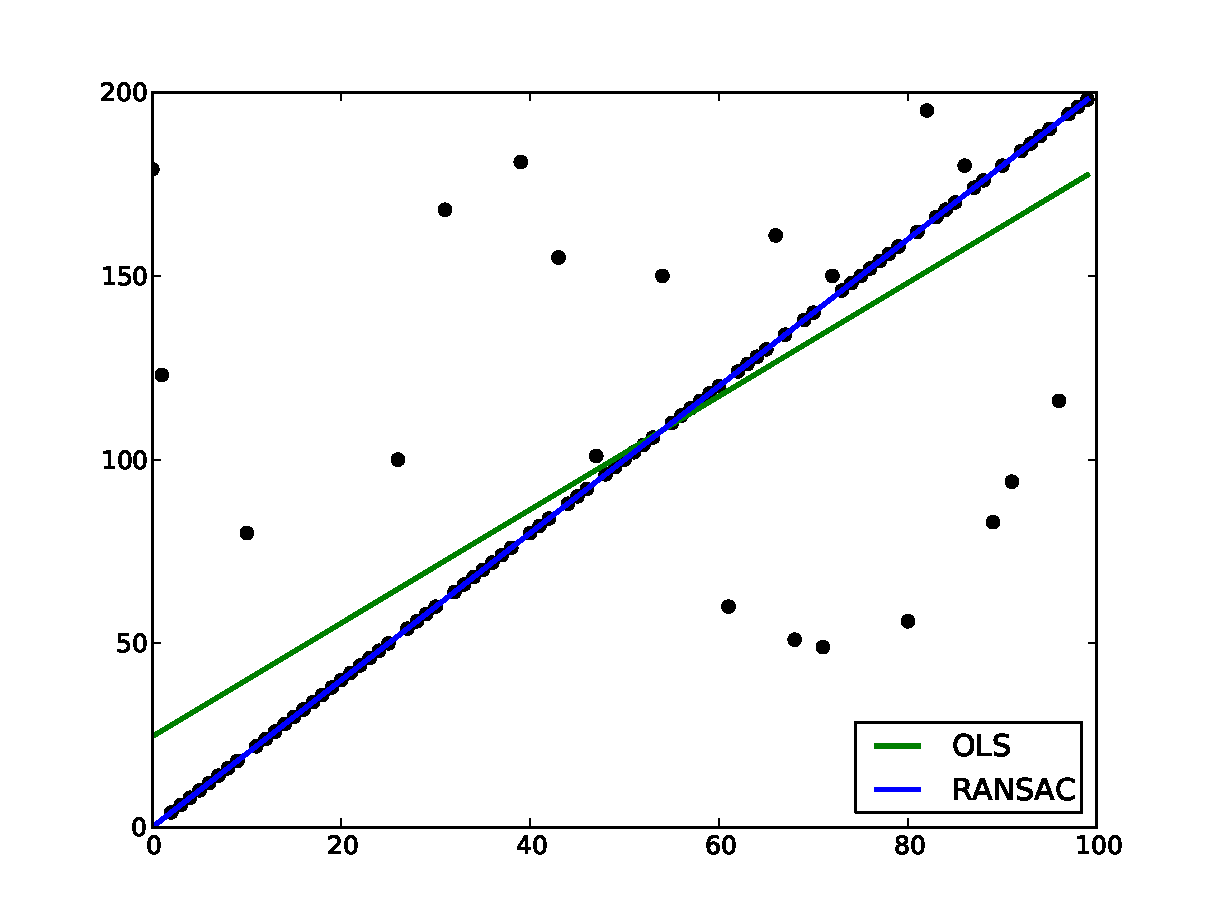
\includegraphics[width=\linewidth]{ransac}
    \caption{RANSAC algorithm in action.}
\end{figure}

\subsection{Sequence alignment}

\section{State inference}

\chapter{Results}

\section{Data sets}

\chapter{Discussion}

\chapter{Conclusions}

\section{Limitations}

\subsection{Textual protocols}

\subsection{Variable number of fields}

\subsection{Non-aligned data}

\subsection{Bit precision}

\section{Future work}

\subsection{Correspondence analysis}

\subsection{Timestamp identification}

\bibliographystyle{plain}
\bibliography{thesis}

\end{document}

